\section{Project Design}
\label{sec:design}

This section explains \emph{how} the project was carried out: the overall approach, the method used for each objective, how the evaluation was designed, and why these methods were chosen.

\subsection{Design and Methods}

\subsubsection*{Research approach}

The project is a \textbf{software development project with an embedded machine-learning experiment}. Its research approach is design-oriented: a working artefact is built to address a real problem, and the artefact is then evaluated to produce evidence about how well the problem is solved. Two kinds of question are asked, and each needs a different method:
\begin{itemize}
  \item \emph{Can the system detect cosmetic concerns reliably?} This is a quantitative question, answered with held-out model metrics.
  \item \emph{Does the finished application work and is it usable?} This is answered with functional tests, an expert heuristic review and a participant survey.
\end{itemize}
The evaluation is therefore \textbf{mixed-methods}, combining numerical model results with structured usability evidence.

\subsubsection*{Development methodology}

Development followed an \textbf{iterative, Agile-inspired process}. Work was organised into short iterations, each ending with a runnable version of the system. Each component (data, model, catalogue, recommender, API, mobile client) was built and tested on its own, then integrated. Evidence from each iteration was allowed to change the plan.

The machine-learning strand followed the \textbf{CRISP-DM} cycle, the most widely used process model for data-mining projects \citep{schroer2021}. Its six phases map directly onto this project:
\begin{enumerate}
  \item \emph{Business understanding:} cosmetic guidance for Nepalese users, without medical claims.
  \item \emph{Data understanding:} the audit of every candidate image source.
  \item \emph{Data preparation:} human review, label definitions and leakage-free splits.
  \item \emph{Modelling:} transfer learning with EfficientNetB0.
  \item \emph{Evaluation:} held-out metrics, with thresholds fixed on validation data.
  \item \emph{Deployment:} serving the model behind the FastAPI backend.
\end{enumerate}
CRISP-DM is explicitly cyclical: an evaluation result can send the project back to data understanding. This happened twice. The first audit replaced disease classification with cosmetic concerns. Later, weak results for the concerns with few negative examples led to a second round of human label review and a retrained model (Figure~\ref{fig:pipeline}).

\begin{figure}[p]
\centering
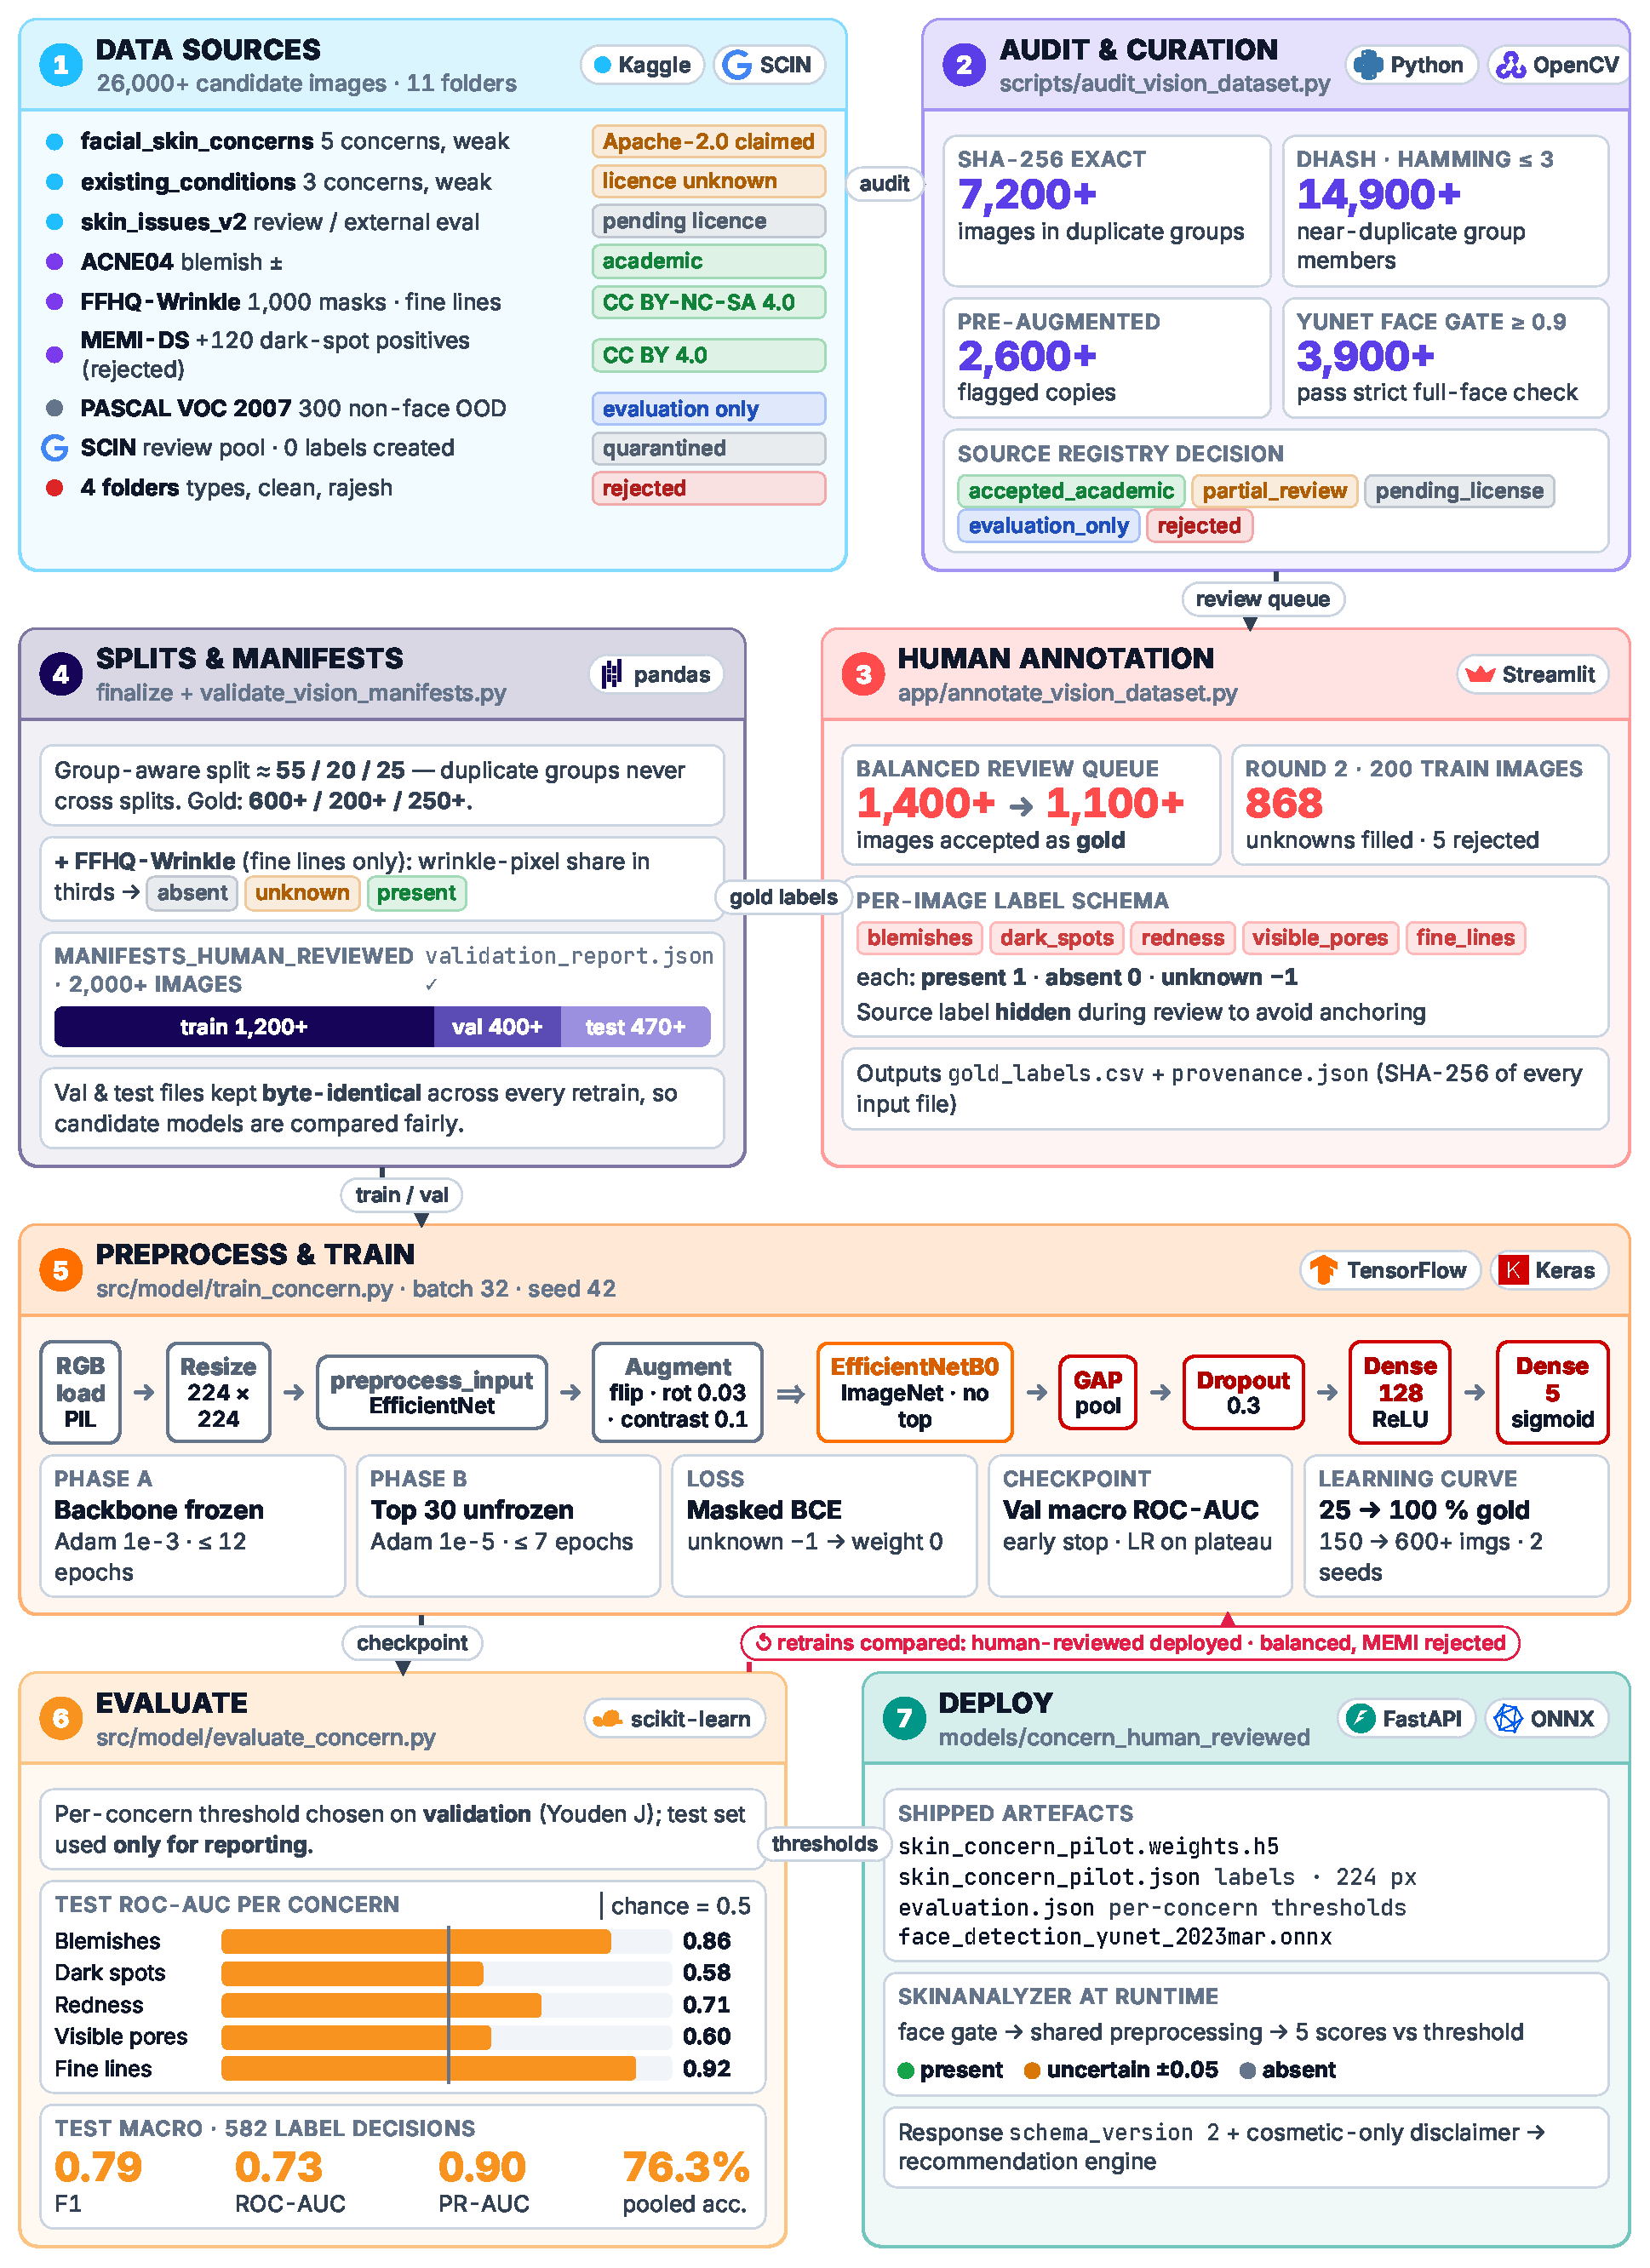
\includegraphics[width=\linewidth]{figures/pipeline.pdf}
\caption{Data and model development pipeline}
\label{fig:pipeline}
\end{figure}

\subsubsection*{Methods for each objective}

Table~\ref{tab:methods} summarises the method, tools and evidence for each objective. The key method details follow the table.

\begin{table}[ht]
\centering\small
\caption{Methods, tools and evidence for each objective}
\label{tab:methods}
\begin{tabularx}{\linewidth}{P{1.9cm}P{3.6cm}P{3.1cm}Y}
\toprule
\textbf{Objective} & \textbf{Method} & \textbf{Main tools} & \textbf{Output and evidence}\\
\midrule
O1 Dataset & Data audit, human annotation, group-aware splitting & SHA-256, dHash, YuNet, Streamlit & Source registry, annotation files, validated manifests\\
O2 Model & Supervised transfer learning, multi-label with masked loss & TensorFlow/Keras, EfficientNetB0 & Weights, \texttt{evaluation.json} with weight hash\\
O3 Catalogue & Web scraping and data cleaning & Python, pandas, rapidfuzz & Unified product CSV\\
O4 Recommender & Rule-based content filtering with a weighted score & Python & Ranked products with matched ingredients\\
O5 Application & Client--server development & FastAPI, Expo/React Native & Running app, API contract tests\\
O6 Evaluation & Mixed methods: metrics, functional tests, heuristic review, survey & unittest, curl, Google Forms & Evidence files, test tables, survey responses\\
\bottomrule
\end{tabularx}
\end{table}

\textbf{Data audit and annotation (O1).} Every candidate image was hashed twice. SHA-256 found exact copies, and a 64-bit difference hash (dHash) with a Hamming radius of 3 found near-duplicates. A YuNet face detector \citep{wu2023yunet} recorded whether each image showed a full face, a close-up or no face. Each source was entered in a registry with its licence, provenance and decision.

Images were then labelled in a purpose-built Streamlit tool, following a written guide (Appendix~\ref{app:annotation}). Each concern was marked \emph{present}, \emph{absent} or \emph{unknown}, and the original folder label was hidden to reduce anchoring bias. A first queue of 1,400+ images was reviewed, followed by a second review of 200 training images whose labels were still unknown. FFHQ-Wrinkle masks \citep{moon2024} were converted to fine-line labels by wrinkle-pixel coverage: the lowest third became absent, the highest third present, and the middle third unknown.

Duplicate groups were assigned to a split as a unit, at roughly 55/20/25. No near-duplicate can therefore appear in both training and testing \citep{barz2020,kapoor2023}.

\textbf{Model training (O2).} The model is an ImageNet-pretrained EfficientNetB0 \citep{tan2019} with a five-output sigmoid head. It is trained with \emph{masked} binary cross-entropy, so unknown labels contribute no gradient and ``not annotated'' is never treated as ``absent'' \citep{liu2022multilabel}. Training has two phases: the head is trained with the backbone frozen (Adam, learning rate $10^{-3}$), then the top 30 layers are fine-tuned (learning rate $10^{-5}$). The final checkpoint is chosen on validation data only.

Each concern's threshold maximises Youden's $J$ (bookmaker informedness) on validation data \citep{chicco2021}. The test set is used only for reporting. Because positives dominate most concerns, balanced accuracy and ROC-AUC are reported next to F1, which on its own rewards always predicting ``present'' \citep{chicco2020}.

\textbf{Catalogue and recommender (O3, O4).} Product pages from Jeevee, ForEveryNG and Oriflame were scraped to CSV and normalised to one schema. Near-duplicate products were merged using \texttt{rapidfuzz} token-sort similarity ($\geq 85$), keeping the most complete record. Category, ingredient and skin-type tags were inferred from keyword dictionaries. Each concern maps to beneficial ingredients and categories (Table~\ref{tab:rules}), and products are ranked by a weighted linear score (Section~\ref{sec:recommender}).

\textbf{Application (O5).} A FastAPI REST backend wraps the model, face gate, recommender and language model. An Expo (React Native) client provides the interface. The two communicate only through a versioned JSON contract that is covered by a unit test.

\subsubsection*{Evaluation design (O6)}

The evaluation has five strands, chosen so that each one covers a weakness of the others:
\begin{enumerate}
  \item \textbf{Held-out model metrics} for every model version, on the same fixed test set.
  \item \textbf{A learning-curve study}, retraining on 25--100\% of the data, to test whether more data would help.
  \item \textbf{Black-box functional tests}: 19 documented cases run against the live API.
  \item \textbf{A heuristic evaluation} of the running app against Nielsen's ten heuristics \citep{galavi2024}.
  \item \textbf{A participant usability survey.} Participants install and use the app, complete four set tasks (check a photo, read the result, find a product, ask the assistant), then answer a Google Form. The form contains consent, anonymous background questions, task completion and ease ratings, the ten-item System Usability Scale \citep{vlachogianni2022}, and questions about trust and understanding of the results. No names, emails or photos are collected. The full protocol is in Appendix~\ref{app:usability}.
\end{enumerate}

\subsection{Justification of Methods}

\textbf{Iterative process and CRISP-DM rather than a fixed plan.} The data's quality was unknown at the start. A fixed, waterfall-style plan would have committed the project to the disease classifier before the audit showed it was unsafe. An iterative process made it possible to change direction on evidence \citep{schroer2021}.

\textbf{Transfer learning rather than training from scratch.} With only 1,200+ training images, a CNN trained from scratch would overfit badly. ImageNet features give a strong starting point for texture and colour \citep{zhuang2021}. EfficientNetB0 was chosen over the planned B2 because it has about 5.3 million parameters, compared with about 9.2 million for B2. On a CPU-only backend, the smaller model's speed outweighed any small accuracy gain that B2 might have given.

\textbf{Multi-label with masking rather than multi-class.} Concerns co-occur on real faces, so a single softmax label would force the model to pick one. Masking lets partially labelled images still contribute: an image labelled only for fine lines still trains the fine-lines output.

\textbf{Audit and human review rather than accepting folder labels.} The folder labels in the Kaggle sources were contaminated (Section~\ref{sec:construction}). Training on them would have produced impressive but meaningless accuracy. Human review is slower, but it is the only way to obtain labels whose meaning is defined.

\textbf{Skin type from the user rather than from the photo.} The only skin-type image source was rejected (100+ images, including stock photographs). Oiliness and dryness are also partly tactile, so they are hard to judge from one photo. Asking the user is more reliable and more respectful.

\textbf{Weighted rules rather than TF-IDF similarity or collaborative filtering.} Collaborative filtering needs interaction histories that do not exist \citep{ricci2022}. TF-IDF over ingredient text was planned, but scraped listings rarely include full ingredient lists: 65\% of products have no inferable ingredient at all. A weighted score over explicit features is simpler, degrades predictably and can be explained line by line \citep{roy2022}.

\textbf{Grounded language model rather than free generation.} Qwen2.5 \citep{qwen2024} runs locally without a paid API. Its outputs are restricted in code, not only by the prompt, to product IDs in the candidate set. It is optional, and the core flow never depends on it. This limits the hallucination risk \citep{ji2023}.

\textbf{Heuristic review and an online survey together.} A heuristic review finds many interface problems cheaply, but it reflects only the evaluator's view \citep{galavi2024}. A survey with SUS captures how real users perceive the app and gives a score that can be compared with published benchmarks \citep{vlachogianni2022}. Google Forms was chosen because it is free, needs no account for participants, records responses anonymously, and exports directly to CSV for analysis.
